%++++++++++++++++++++++++++++++++++++++++
\documentclass[article, 12pt]{article}
\usepackage{float}
\usepackage{setspace}
\usepackage{tabu} % extra features for tabular environment
\usepackage{amsmath}  % improve math presentation
\usepackage{graphicx} % takes care of graphic including machinery
\usepackage[margin=1in]{geometry} % decreases margins
\usepackage{cite} % takes care of citations
\usepackage[final]{hyperref} % adds hyper links inside the generated pdf file
\usepackage{tikz}
\usepackage{caption} 
\usepackage{fancyhdr}
\usepackage{amssymb} % symbols like /therefore
\usepackage{amsthm} % proofs
\usepackage{enumerate} % lettered lists
\usepackage{mathtools} % macros
\usepackage[all]{xy} % for diagrams
\usepackage{tkz-graph}
\usetikzlibrary{knots}
\usepackage{xcolor}
\usetikzlibrary{scopes}
% \usepackage{xcolor} \pagecolor[rgb]{0.12549019607,0.1294117647,0.13725490196} \color[rgb]{0.82352941176,0.76862745098,0.62745098039} % dark theme
\theoremstyle{definition}
\newtheorem{example}{Example}[subsubsection]
\newtheorem*{remark}{Remark}
\newtheorem{theorem}{Theorem}[subsubsection]
\newtheorem{definition}{Definition}
\newtheorem{corollary}{Corollary}[subsubsection]
\hypersetup{
	colorlinks=false,      % false: boxed links; true: colored links
	linkcolor=blue,        % color of internal links
	citecolor=blue,        % color of links to bibliography
	filecolor=magenta,     % color of file links
	urlcolor=blue         
}
\usepackage{physics}
\usepackage{siunitx}
\usepackage{tikz,pgfplots}
\usepackage[outline]{contour} % glow around text
\usetikzlibrary{calc}
\usetikzlibrary{angles,quotes} % for pic
\usetikzlibrary{arrows.meta}
\tikzset{>=latex} % for LaTeX arrow head
\contourlength{1.2pt}

\colorlet{xcol}{blue!70!black}
\colorlet{vcol}{green!60!black}
\colorlet{myred}{red!70!black}
\colorlet{myblue}{blue!70!black}
\colorlet{mygreen}{green!70!black}
\colorlet{mydarkred}{myred!70!black}
\colorlet{mydarkblue}{myblue!60!black}
\colorlet{mydarkgreen}{mygreen!60!black}
\colorlet{acol}{red!50!blue!80!black!80}
\tikzstyle{CM}=[red!40!black,fill=red!80!black!80]
\tikzstyle{xline}=[xcol,thick,smooth]
\tikzstyle{mass}=[line width=0.6,red!30!black,fill=red!40!black!10,rounded corners=1,
                  top color=red!40!black!20,bottom color=red!40!black!10,shading angle=20]
\tikzstyle{faded mass}=[dashed,line width=0.1,red!30!black!40,fill=red!40!black!10,rounded corners=1,
                        top color=red!40!black!10,bottom color=red!40!black!10,shading angle=20]
\tikzstyle{rope}=[brown!70!black,very thick,line cap=round]
\def\rope#1{ \draw[black,line width=1.4] #1; \draw[rope,line width=1.1] #1; }
\tikzstyle{force}=[->,myred,very thick,line cap=round]
\tikzstyle{velocity}=[->,vcol,very thick,line cap=round]
\tikzstyle{Fproj}=[force,myred!40]
\tikzstyle{myarr}=[-{Latex[length=3,width=2]},thin]
\def\tick#1#2{\draw[thick] (#1)++(#2:0.12) --++ (#2-180:0.24)}
\DeclareMathOperator{\sn}{sn}
\DeclareMathOperator{\cn}{cn}
\DeclareMathOperator{\dn}{dn}
\def\N{80} % number of samples in plots


\usepackage{titling}
\renewcommand\maketitlehooka{\null\mbox{}\vfill}
\renewcommand\maketitlehookd{\vfill\null}
\usepackage{siunitx} % units
\usepackage{verbatim} 
\newcommand{\courseNumber}{MATH 1700}
\newcommand{\courseName}{Ideas in Mathematics}
\newcommand{\professor}{Professor Rimmer}
\newcommand{\psetName}{Worksheet 11: Euler Cycles Second Submission}
\newcommand{\dueDate}{Due: April 19, 2023}
\newcommand{\name}{Denny Cao}
\pagestyle{fancy}
\fancyhf{}% clears all header and footer fields
\fancyfoot[C]{--~\thepage~--}
\renewcommand*{\headrulewidth}{0.4pt}
\renewcommand*{\footrulewidth}{0pt}
\lhead{\name}
\chead{\courseNumber: \courseName}
\rhead{\professor}

% new theorem for questions and answers

\newtheorem{question}{Question}

\newtheorem{answer}{Answer}

\fancypagestyle{plain}{%
  \fancyhf{}% clears all header and footer fields
  \fancyfoot[C]{--~\thepage~--}%
  \renewcommand*{\headrulewidth}{0pt}%
  \renewcommand*{\footrulewidth}{0pt}%
}

% Shortcuts
\DeclarePairedDelimiter\ceil{\lceil}{\rceil} % ceil function
\DeclarePairedDelimiter\floor{\lfloor}{\rfloor} % floor function

\DeclarePairedDelimiter\paren{(}{)} % parenthesis

\newcommand{\df}{\displaystyle\frac} % displaystyle fraction
\newcommand{\qeq}{\overset{?}{=}} % questionable equality

\newcommand{\Mod}[1]{\;\mathrm{mod}\; #1} % modulo operator

\newcommand{\comp}{\circ} % composition

% Sets
\DeclarePairedDelimiter\set{\{}{\}}
\newcommand{\unite}{\cup}
\newcommand{\inter}{\cap}

\newcommand{\reals}{\mathbb{R}} % real numbers: textbook is Z^+ and 0
\newcommand{\ints}{\mathbb{Z}}
\newcommand{\nats}{\mathbb{N}}
\newcommand{\rats}{\mathbb{Q}}

\newcommand{\degree}{^\circ}

% Counting
\newcommand\perm[2][^n]{\prescript{#1\mkern-2.5mu}{}P_{#2}}
\newcommand\comb[2][^n]{\prescript{#1\mkern-0.5mu}{}C_{#2}}

% Relations
\newcommand{\rel}{\mathcal{R}} % relation

\setlength\parindent{0pt}

% Directed Graphs
\usetikzlibrary{arrows}
\tikzset{vertex/.style = {shape=circle,draw,minimum size=2em}}
\tikzset{svertex/.style = {shape=circle,draw,minimum size=.05em,font=\tiny}}
\tikzset{edge/.style = {->,> = latex'}}
\tikzset{dedge/.style = {-> = latex'}}
\tikzset{dot/.style={inner sep=1.5pt,circle,draw,fill}}

% Contradiction
\newcommand{\contradiction}{{\hbox{%
    \setbox0=\hbox{$\mkern-3mu\times\mkern-3mu$}%
    \setbox1=\hbox to0pt{\hss$\times$\hss}%
    \copy0\raisebox{0.5\wd0}{\copy1}\raisebox{-0.5\wd0}{\box1}\box0
}}}

% Sign Charts
\newdimen\tcolw \tcolw=2.5em % the column width
\edef\ecatcode{\catcode`&=\the\catcode`&\relax}\catcode`&=4
\def\sgchart#1#2{\vbox{\offinterlineskip\halign{\hfil##\quad&##\hfil\crcr\sgchartA#2,:,%
   \omit\sgchartR&\kern.2pt\sgchartS{.5\tcolw}\relax\sgchartE#1,\relax,%
   \sgchartS{.5\tcolw}\relax\cr
   \noalign{\kern2pt}&\def~{}\kern.5\tcolw\sgchartD#1,\relax,\cr}}}
\def\sgchartA#1:#2,{\cr\ifx,#1,\else $#1$&\sgchartB#2{}\expandafter\sgchartA\fi}
\def\sgchartB#1{\hbox to\tcolw{\hss$#1$\hss}\sgchartC}
\def\sgchartC#1{\ifx,#1,\else
   \strut\vrule\kern-.4pt\hbox to\tcolw{\hss$#1$\hss}\expandafter\sgchartC\fi}
\def\sgchartD#1#2,{\ifx\relax#1\else\hbox to\tcolw{\hss$#1#2$\hss}\expandafter\sgchartD\fi}
\def\sgchartE#1#2,{\ifx\relax#1\else
    \ifx~#1\sgchartS\tcolw\circ \else\sgchartS\tcolw\bullet\fi \expandafter\sgchartE\fi}
\def\sgchartR{\leaders\vrule height2.8pt depth-2.4pt\hfil}
\def\sgchartS#1#2{\hbox to#1{\kern-.2pt\sgchartR \ifx\relax#2\else
   \kern-.7pt$#2$\kern-.7pt\sgchartR\fi\kern-.2pt}}
\ecatcode
%++++++++++++++++++++++++++++++++++++++++
% title stuff

\makeatletter
\renewcommand{\maketitle}{\bgroup\setlength{\parindent}{0pt}
    \begin{flushleft}
        \textbf{\@title} \\ \vskip0.2cm
        \begingroup
            \fontsize{14pt}{12pt}\selectfont
            \courseNumber: \courseName 
            \vskip0.3cm 
            \professor
        \endgroup \vskip0.3cm
        \dueDate \hfill\rlap{}\bf{\name} \\ \vskip0.1cm
        \hrulefill
    \end{flushleft}\egroup 
}
\makeatother

\title{\Large\bf{\psetName}}

\begin{document}
    \maketitle
    \thispagestyle{plain}
    \section{Warm-Up}
    % Question 1
    \begin{question}
        Cycle City consists of four islands, labeled $A$, $B$, $C$, and $D$. There are various bridges to help the residents get from island to island. The map is pictured below. The circles represent the islands, and the lines between circles (some curved, some straight) represent the bridges between islands.
        \begin{figure}[H]
            \centering
            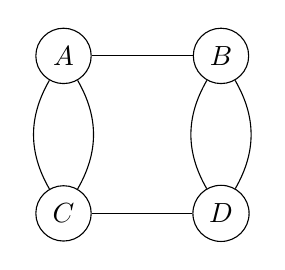
\begin{tikzpicture}
                \node[vertex] (A) at (0,0) {$A$};
                \node[vertex] (B) at (2,0) {$B$};
                \node[vertex] (C) at (0,-2) {$C$};
                \node[vertex] (D) at (2,-2) {$D$};

                \draw (A) -- (B);
                \draw (C) -- (D);

                \draw (A) to[bend left] (C);
                \draw (A) to[bend right] (C);

                \draw (B) to[bend left] (D);
                \draw (B) to[bend right] (D);
            \end{tikzpicture}
        \end{figure}
        The mayor of Cycle City, Bob the Bicyclist, would like to find a way to start at Island
        A, then bike around the island, using every bridge exactly once, so that he ends up back on Island A. Unfortunately, this is not possible. Write a short note (a few sentences) to Bob the Bicyclist explaining why he can't achieve his goal. Bob was educated at Calculus College, where he didn't learn anything about graph theory, so you should define and state any graph-theoretic terms and theorems you use.
    \end{question}
    % Answer 1
    \begin{answer}
        \begin{proof}
            Hey Bob! Your goal is to find an Euler circuit, a path that uses every edge---bridge---exactly once. By the Euler's Cycle Theorem, an Euler circuit exists if and only if every vertex---island---has an even degree---number of bridges. In this case, each island has a degree of 3. As there exists a vertex with an odd degree, there cannot be an Euler circuit.
        \end{proof}
    \end{answer}
    \section{More About Euler Cycles}
    % Question 2
    \begin{question}
        After receiving your initial correspondence, Bob the Bicyclist (from Problem 1) decides he would like to add some bridges to Cycle City so that he can start at Island A, bike around, using every bridge exactly once, and end up at A again. How many new bridges must he build? For full credit, explain why your answer is optimal (i.e., why you couldn't get away with fewer new bridges, which Bob would certainly want to be sure of before starting the project).
    \end{question}
    % Answer 2
    \begin{answer}
        \begin{proof}
            Bob needs to add 2 new bridges. The reason for this is that the degree of each vertex must be even. In this case, each vertex has a degree of 3. If we add 2 new bridges, as follows:
            \begin{figure}[H]
                \centering
                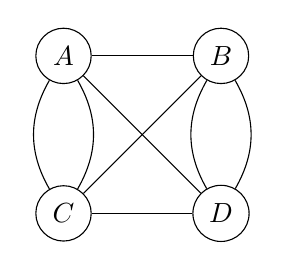
\begin{tikzpicture}
                    \node[vertex] (A) at (0,0) {$A$};
                    \node[vertex] (B) at (2,0) {$B$};
                    \node[vertex] (C) at (0,-2) {$C$};
                    \node[vertex] (D) at (2,-2) {$D$};
    
                    \draw (A) -- (B);
                    \draw (C) -- (D);
    
                    \draw (A) to[bend left] (C);
                    \draw (A) to[bend right] (C);
    
                    \draw (B) to[bend left] (D);
                    \draw (B) to[bend right] (D);

                    \draw (A) -- (D);
                    \draw (B) -- (C);
                \end{tikzpicture}
            \end{figure}
            then each vertex has a degree of 4, which is even. Thus, there is an Euler circuit. This is the optimal number of bridges, as by adding 1, only 2 vertices would have an even degree.
        \end{proof}
    \end{answer}
    % Question 3
    \begin{question}
        The following multigraph has an Euler cycle. Explain how you can tell that this is the case, without actually finding an Euler cycle.
        \begin{figure}[H]
            \centering
            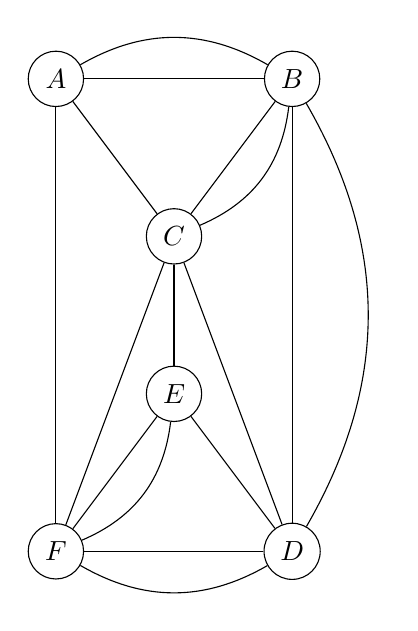
\begin{tikzpicture}
                \node[vertex] (A) at (0,0) {$A$};
                \node[vertex] (B) at (3,0) {$B$};
                \node[vertex] (D) at (3,-6) {$D$};
                \node[vertex] (F) at (0,-6) {$F$};
                \node[vertex] (C) at (1.5,-2) {$C$};
                \node[vertex] (E) at (1.5,-4) {$E$};

                \draw (A) -- (B);
                \draw (A) to[bend left] (B);
                \draw (A) -- (F);
                \draw (A) -- (C);
                \draw (B) -- (C);
                \draw (B) to[bend left] (C);
                \draw (B) -- (D);
                \draw (B) to[bend left] (D);
                \draw (C) -- (E);
                \draw (E) -- (F);
                \draw (E) to[bend left] (F);
                \draw (E) -- (D);
                \draw (F) -- (D);
                \draw (C) -- (D);
                \draw (F) -- (C);
                \draw (F) to[bend right] (D);
            \end{tikzpicture}
        \end{figure}
    \end{question}
    % Answer 3
    \begin{answer}
        \begin{proof}
            The degree of each vertex is as follows:
            \begin{figure}[H]
                \centering
                \begin{tabular}{|c|c|}
                    \hline
                    Vertex & Degree \\
                    \hline
                    A & 4 \\
                    B & 6 \\
                    C & 6 \\
                    D & 6 \\
                    E & 4 \\
                    F & 6 \\
                    \hline
                \end{tabular}
            \end{figure}
            As each vertex has an even degree, there is an Euler cycle.
        \end{proof}
    \end{answer}
    % Question 4
    \begin{question}
        Use the algorithm described in the videos to find an Euler cycle for the multigraph in Problem 3. In the first step, you use the mini-cycle $AF$, $FC$, $CA$, $AB$, $BA$. Be sure to explain the steps of the process, as they correspond to the steps outlined in the videos.
    \end{question}
    % Answer 4
    \begin{answer} \ \\
        The mini-cycle is as follows in red:
        \begin{figure}[H]
            \centering
            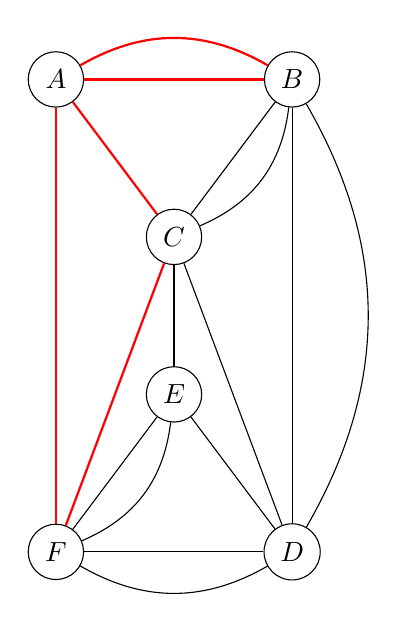
\begin{tikzpicture}
                \node[vertex] (A) at (0,0) {$A$};
                \node[vertex] (B) at (3,0) {$B$};
                \node[vertex] (D) at (3,-6) {$D$};
                \node[vertex] (F) at (0,-6) {$F$};
                \node[vertex] (C) at (1.5,-2) {$C$};
                \node[vertex] (E) at (1.5,-4) {$E$};

                
                \draw[thick, red] (A) -- (B);
                \draw[thick, red] (A) to[bend left] (B);
                \draw[thick, red] (A) -- (F);
                \draw[thick, red] (A) -- (C);
                \draw[thick, red] (F) -- (C);

                \draw (B) -- (C);
                \draw (B) to[bend left] (C);
                \draw (B) -- (D);
                \draw (B) to[bend left] (D);
                \draw (C) -- (E);
                \draw (E) -- (F);
                \draw (E) to[bend left] (F);
                \draw (E) -- (D);
                \draw (F) -- (D);
                \draw (C) -- (D);
                \draw (F) to[bend right] (D);
            \end{tikzpicture}
        \end{figure}
        \textbf{Step 1: List all (remaining) edges in the graph.}

        The remaining edges are: 
        $EC$, $EF$, $FE$, $FD$, $DF$, $DE$, $DC$, $BC$, $CB$, $BD$, $DB$.

        \textbf{Step 2: Choose a vertex in the list. Make a path from that vertex using edges from that list, stopping when you get stuck. This is a mini-cycle.}

        We pick vertex $C$. Using the edges from Step 1, we get the mini-cycle $CB$, $BC$, $CE$, $EF$, $FD$, $DF$, $FE$, $ED$, $DB$, $BD$, $DC$. This mini-cycle is in blue in the figure below:
        \begin{figure}[H]
            \centering
            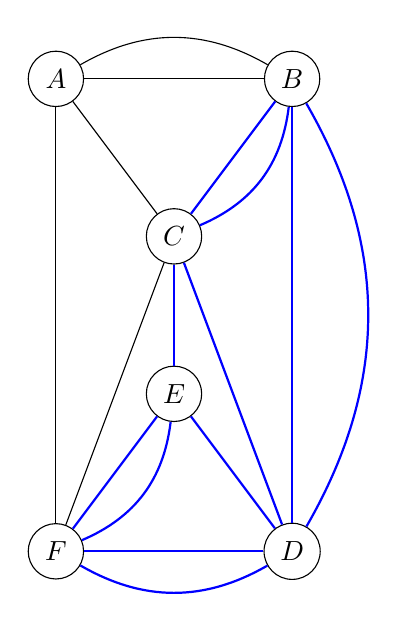
\begin{tikzpicture}
                \node[vertex] (A) at (0,0) {$A$};
                \node[vertex] (B) at (3,0) {$B$};
                \node[vertex] (D) at (3,-6) {$D$};
                \node[vertex] (F) at (0,-6) {$F$};
                \node[vertex] (C) at (1.5,-2) {$C$};
                \node[vertex] (E) at (1.5,-4) {$E$};

                
                \draw (A) -- (B);
                \draw (A) to[bend left] (B);
                \draw (A) -- (F);
                \draw (A) -- (C);
                \draw (F) -- (C);

                \draw[thick, blue] (B) -- (C);
                \draw[thick, blue] (B) to[bend left] (C);
                \draw[thick, blue] (B) -- (D);
                \draw[thick, blue] (B) to[bend left] (D);
                \draw[thick, blue] (C) -- (E);
                \draw[thick, blue] (E) -- (F);
                \draw[thick, blue] (E) to[bend left] (F);
                \draw[thick, blue] (E) -- (D);
                \draw[thick, blue] (F) -- (D);
                \draw[thick, blue] (C) -- (D);
                \draw[thick, blue] (F) to[bend right] (D);
            \end{tikzpicture}
        \end{figure}
        \textbf{Step 3: Are there any edges in the list that are not in the mini-cycle? If so, repeat starting at Step 1 with the remaining edges.}
        
        As there are no edges in the list that are not in the mini-cycle, we can proceed to Step 4.
        
        \textbf{Step 4: Splice together the mini-cycles.}

        {\color{red} First mini-cycle: $AF$, $FC$, $CA$, $AB$, $BA$}

        {\color{blue} Second mini-cycle: $CB$, $BC$, $CE$, $EF$, $FD$, $DF$, $FE$, $ED$, $DB$, $BD$, $DC$}
        \\[12pt]
        We splice by placing the second mini-cycle within the first mini-cycle. We get the following Euler cycle: {\color{red} $AF$, $FC$,} {\color{blue}$CB$, $BC$, $CE$, $EF$, $FD$, $DF$, $FE$, $ED$, $DB$, $BD$, $DC$,} {\color{red}$CA$, $AB$, $BA$}.

    \end{answer}
    % Question 5
    \begin{question}
        The city of Bridgelandia consists of five islands, named A, B, C, D, and E, with bridges connecting them. It is possible to travel between any two islands.
        \\[12pt]
        You are a tourist who wants to see as much of the city as possible. You begin at Island $A$, and walk around somewhat aimlessly. However, you make sure never to use the same bridge twice. At some point, you get stuck---you arrive on some island, and there are no new bridges from that island to take. Given the additional information that Island $C$ has exactly four bridges connecting it to other islands, explain why it is impossible that you got stuck on Island $C$.
    \end{question}
    % Answer 5
    \begin{answer}
        \begin{proof} By contradiction.
            Assume for the purposes of contradiction that you got stuck on Island $C$. This means that you have used all the bridges connected to Island $C$ and there is no new bridge to take. Since Island $C$ has four bridges connecting it to other islands, let us label these bridges as $C_1, C_2, C_3$, and $C_4$. Without loss of generality, let us assume that you arrived at Island $C$ using bridge $C_1$. This means that you have used bridges $C_2$, $C_3$, and $C_4$ to reach other islands.

            Now, consider the three islands connected to Island $C$ by bridges $C_2$, $C_3$, and $C_4$. Let these islands be denoted by $X$, $Y$, and $Z$. Since you have used all the bridges connected to Island $C$, you cannot use any of the bridges $C_2$, $C_3$, or $C_4$ to leave Island $X$, $Y$, or $Z$ respectively. Therefore, you must use the bridge connecting Island $X$ and Island $Y$, the bridge connecting Island $Y$ and Island $Z$, and the bridge connecting Island $Z$ and Island $X$. $\contradiction$
            \\[12pt]
            However, this means that you will have to use the bridge $C_1$ to leave Island $C$, which contradicts the assumption that you got stuck on Island $C$ without using all the bridges connected to it. Therefore, it is impossible that you got stuck on Island $C$.
        \end{proof}
    \end{answer}
    \section{Euler Paths}
    % Question 6
    \begin{question}
        Define what it means for a path on a (multi)graph to be an \textit{Euler path}.
    \end{question}
    % Answer 6
    \begin{answer}
        \begin{definition}
            A path on a (multi)graph is an Euler path if it uses every edge and every vertex exactly once. A multigraph has an Euler path but not an Euler circuit if and only if it has exactly two vertices of odd degree.
        \end{definition}
    \end{answer}
    % Question 7
    \begin{question}
        Explain why the following multigraph does not have an Euler cycle. Does it have an Euler path? If so, find one.
        \begin{figure}[H]
            \centering
            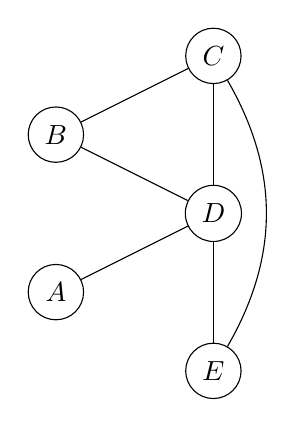
\begin{tikzpicture}
                \node[vertex] (A) at (0,0) {$A$};
                \node[vertex] (B) at (0,2) {$B$};
                \node[vertex] (C) at (2,3) {$C$};
                \node[vertex] (D) at (2,1) {$D$};
                \node[vertex] (E) at (2,-1) {$E$};

                \draw (B) -- (C);
                \draw (B) -- (D);
                \draw (A) -- (D);
                \draw (E) -- (D);
                \draw (D) -- (C);
                \draw (C) to[bend left] (E);
            \end{tikzpicture}
        \end{figure}
    \end{question}
    % Answer 7
    \begin{answer}
        \begin{proof}
             The vertex $A$ has degree 1, which is odd. As there exists a vertex of odd degree, the multigraph does not have an Euler cycle.
            \\[12pt]
            The multigraph has an Euler path. There are exactly two vertices of odd degree, $A$ with degree of 1, and $D$ with degree of 3. Since there are exactly two vertices of odd degree, the multigraph has an Euler path. We can find an Euler path by starting at vertex $A$ and following the edges in the order $AD$, $DB$, $BC$, $CE$, $ED$, $DC$.
        \end{proof}
    \end{answer}
    % Question 8
    \begin{question}
        Your friend fell asleep after watching a Math 170 video, and had a dream about a multigraph. They tell you this multigraph had four vertices, labeled $A$, $B$, $C$, and $D$, and that it was connected. They also tell you that vertices $A$ and $D$ both had odd degree, and vertices $B$ and $C$ both had even degree. Without knowing anything more, explain why it's possible to add a single edge to the multigraph so that the resulting multigraph has an Euler cycle.
    \end{question}
    % Answer 8
    \begin{answer}
        By adding an edge from $A$ to $D$, we can increase the degree of both by 1. This means that the degree of both are now even, and this new edge does not change the degree of $B$ and $C$. As all the vertices now have even degree, the resulting multigraph has an Euler cycle.
    \end{answer}
    % Question 9
    \begin{question}
        Explain why the original multigraph in your friend's dream (from Problem 8) must have
        an Euler path.        
    \end{question}
    % Answer 9
    \begin{answer}
        There are two vertices of odd degree, $A$ and $D$. Since there are exactly two vertices of odd degree, the multigraph has an Euler path.
    \end{answer}
    \section{Hamiltonian Paths and Cycles}
    % Question 10
    \begin{question}
        Go online and look up the definition of Hamiltonian paths and Hamiltonian cycles. What is the difference between a Hamiltonian path and an Euler path? What is the difference between a Hamiltonian cycle and an and an Euler cycle?
    \end{question}
    % Answer 10
    \begin{answer}
        \begin{definition}
            A \textbf{Hamiltonian path} is a path that visits every vertex exactly once. A \textbf{Hamiltonian cycle} is a path that visits every vertex exactly once and returns to the starting vertex.
        \end{definition}
        \begin{definition}
            An \textbf{Euler path} is a path that uses every edge exactly once. An \textbf{Euler cycle} is a path that uses every edge exactly once and returns to the starting vertex. 
        \end{definition} 
        The difference between a Hamiltonian path and an Euler path is that a Hamiltonian path visits every \textit{vertex} exactly once, while an Euler path uses every \textit{edge} exactly once. The difference between a Hamiltonian cycle and an Euler cycle is that a Hamiltonian cycle visits every vertex exactly once and returns to the starting vertex, while an Euler cycle uses every edge exactly once and returns to the starting vertex.
    \end{answer}
    % Question 11
    \begin{question}
        Suppose you are visiting an amusement park, and you want to ride every ride once. Do you want an Euler path or a Hamiltonian path?
    \end{question}
    % Answer 11
    \begin{answer}
        You want a Hamiltonian path because you want to visit every vertex exactly once. You do not care about the edges, so you do not need an Euler path.
    \end{answer}
    % Question 12
    \begin{question}
        Suppose you are visiting a national park, and want to hike the entire system of trails
        without repeating any part of the hike. Do you want an Euler path or a Hamiltonian
        path? What advantage might there be to finding an Euler/Hamiltonian cycle rather than
        an Euler/Hamiltonian path?
    \end{question}
    % Answer 12
    \begin{answer}
        You want an Euler path because you want to visit all trails exactly once. The advantage of finding an Euler cycle is that you are able to visit all the trails and the advantage of finding a Hamiltonian cycle is that you are able to visit all the points of interest but not necessarily all the trails.
    \end{answer}
    % Question 13
    \begin{question}
        Which of the graphs on this worksheet have Hamiltonian paths? Hamiltonian cycles? In each case, either find such a path/cycle or explain how you know there is none.
    \end{question}
    % Answer 13
    \begin{answer}
        Question 1 contains a Hamiltonian path: $AC$, $CD$, $DB$.
        \\[12pt]
        Question 3 contains a Hamiltonian path: $AF$, $FE$, $EC$, $CB$, $BD$.
        \\[12pt]
        Question 7 contains a Hamiltonian path: $AD$, $DB$, $BC$, $CE$.
    \end{answer}
    % Question 14
    \begin{question}
        Explain why any graph that has an Hamiltonian cycle also has a Hamiltonian path. Can you find a graph that has a Hamiltonian path but no Hamiltonian cycle? What happens if you replace the word “Hamiltonian” with “Euler” in this problem?
    \end{question}
    % Answer 14
    \begin{answer}
        Any graph that has a Hamiltonian cycle also has a Hamiltonian path because a Hamiltonian cycle is a Hamiltonian path that starts and ends at the same vertex. A graph that has a Hamiltonian path but no Hamiltonian cycle can be made by leaving 1 vertex with only degree 1. If you replace the word “Hamiltonian” with “Euler” in this problem, you can find a graph that has an Euler path but no Euler cycle. 
    \end{answer}
    % Question 15
    \begin{question}
        Suppose you have a graph with three vertices of degree one, on vertex of degree two, and one vertex of degree three. Can your graph have a Hamiltonian path or a Hamiltonian cycle? Why or why not?
    \end{question}
    % Answer 15
    \begin{answer}
        Your graph cannot have a Hamiltonian path or a Hamiltonian cycle because, once you traverse to a vertex of degree 1, you cannot traverse to any other vertex. 
    \end{answer}
    % Question 16
    \begin{question}
        Suppose you have a graph in which every vertex has degree two. Under what circumstances will the graph have a Hamiltonian path and/or cycle?
    \end{question}
    % Answer 16
    \begin{answer}
        The graph will always have a Hamiltonian cycle, and thus a Hamiltonian path as well. 

        \begin{proof}
            A graph in which every vertex has degree two is a cycle graph, $C_n$. With any cycle, it is possible traverse ``around'' the cycle clockwise or counter-clockwise as follows: $v_1 \rightarrow v_2 \rightarrow v_3 \rightarrow \cdots \rightarrow v_n \rightarrow v_1$. This is a Hamiltonian cycle. By stopping at $v_n$ instead of $v_1$, we can get a Hamiltonian path.
        \end{proof}
    \end{answer}
    \section{Reflection}
    \textbf{Identify at least one wrong or failed idea that turned out to be helpful or enlightening in some way. For instance, that idea might have helped you solve a problem, or it may have been the start of a conversation that improved your understanding more generally. You can list one of your own ideas, or an idea that originated with a classmate. (Please give your classmate credit!)}

    I didn't completely remember the algorithm to find Euler circuits. Rewatching the video refreshed my memory and helped me solve the problem.
\end{document} 
